\newcommand{\pie}[1]{%
\begin{tikzpicture}
 \draw (0,0) circle (1ex);\fill (1ex,0) arc (0:#1:1ex) -- (0,0) -- cycle;
\end{tikzpicture}%
}

\newcommand{\revpie}{%
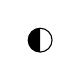
\begin{tikzpicture}
 \draw (0,0) circle (1ex);\fill (0,1ex) arc (90:270:1ex) -- (0,0) -- cycle;
\end{tikzpicture}%
}

\newcommand{\rot}[1]{\rotatebox{#1}}
\newcommand{\CIRCLE}{\pie{360}}
\newcommand{\Circle}{\pie{0}}
\newcommand{\LEFTcircle}{\pie{180}}
\newcommand{\RIGHTcircle}{\revpie}


\begin{table}
    \newcommand{\rh}[1]{\rot{33}{\textbf{#1}}}
    \newcommand{\yes}{\CIRCLE}
    \newcommand{\pa}{\LEFTcircle}
    \newcommand{\no}{\Circle}
    \newcommand{\na}{\makebox[8pt][c]{\textbf{--}}}
    \newcommand{\po}{{\LEFTcircle}}
    \newcommand{\tzfootnote}{\textsuperscript{a}}
    \newcommand{\tzfootnotetext}{We consider TrustZone with the OP-TEE OS and our extensions for attestation}

    \newcolumntype{a}{p{5mm}}
    \setlength{\tabcolsep}{1mm}

     \label{tbl:tee-comparison}
      \resizebox{0.7\textwidth}{!}{
	    \begin{tabular}{@{}l@{\hskip 5mm}aaaaaaa@{\hskip 15mm}aaaa@{\hskip 15mm}r@{}}
	        & \rh{Isolation} & \rh{SW Attestation} & \rh{TCB Attestation} & \rh{Memory Protection} &  \rh{Sealing} & \rh{Code Confidentiality} & \rh{Secure I/O} & \rh{HW-Only TCB} & \rh{Upgradeable TCB} & \rh{Preemption} & \rh{Dynamic Layout}  & \textbf{Target ISA} \\ \midrule
            \textbf{Sancus}                 & \yes & \yes & \yes  & \no  & \no  & \po  & \yes & \yes & \no  & \po  & \no  & MSP430 (16-bit) \\ \midrule
            \textbf{SGX}                    & \yes & \yes & \yes  & \yes & \po  & \po  & \po  & \no  & \yes & \yes & \yes & x86\_64 (64-bit) \\ \midrule
            \textbf{TrustZone\tzfootnote}   & \yes & \yes & \yes  & \no  & \po  & \po  & \po  & \no  & \yes & \yes & \yes & ARM (32-bit) \\
	        \bottomrule \\
    	    \multicolumn{13}{c}{\yes\xspace= Yes; \po\xspace= Possible; \no\xspace= No} \\
	    \end{tabular}
	}

    \caption{Comparison of \ac{TEE} hardware features and the resulting security
    guarantees and application capabilities in our framework. This table is
    derived and adapted from~\cite{maene:hardware}.
    \emph{Footnotes --- } 
    \tzfootnote{}: \tzfootnotetext.
    \vspace{-1em}
   }
\end{table}

